\documentclass[hyperref={pdfpagelabels=false}]{beamer}

\usetheme{Heidelberg}

\usepackage{wrapfig}
\usepackage{lmodern}
\usepackage{natbib}
\usepackage{amsmath,amsfonts,amssymb}
\usepackage{algorithm,algorithmic}
%\floatname{algorithm}{Algorithmus}

%\usepackage{tikz}
%	\usetikzlibrary[topaths,arrows,calc]
\usepackage{wrapfig}
\usepackage{graphicx}
\usepackage{subcaption}


\usepackage[english]{babel}
\usepackage[T1]{fontenc} % Ligaturen, richtige Umlaute im PDF 
\usepackage[utf8]{inputenc}% UTF8-Kodierung für Umlaute usw

\usepackage{hyperref}

\definecolor{darkred}{rgb}{110,1,1}  
\definecolor{maroon}{rgb}{0.5,0,0}  

\newcounter{saveenumi}
\newcommand{\seti}{\setcounter{saveenumi}{\value{enumi}}}
\newcommand{\conti}{\setcounter{enumi}{\value{saveenumi}}}


% zusaetzlich ist das usepackage{beamerthemeshadow} eingebunden 
\usepackage{beamerthemeshadow}

\renewcommand{\thefootnote}{\fnsymbol{footnote}} 

%--------------------------------------------------------------------------%
%--------------------------------------------------------------------------%
%--------------------------------------------------------------------------%
\title[Application of graph matching in Computer Vision]
	{Application of graph matching in Computer Vision}
\subtitle{Master Seminar}
\author[E.~Tikhoncheva] % (optional, for multiple authors)
	{Ekaterina~Tikhoncheva}
\institute[Universities Here and There] % (optional)
	{University of Heidelberg\\
	Faculty of Mathematics and Computer Science \\
	Computer Vision group \\
	at\\
	Heidelberg Collaboratory for Image Processing
}
\date[2015]{November 2015}
%--------------------------------------------------------------------------%
%--------------------------------------------------------------------------%
%--------------------------------------------------------------------------%
\begin{document}
\begin{frame}
\titlepage
\end{frame}
%--------------------------------------------------------------------------%
\begin{frame}
\frametitle{Agenda}
\tableofcontents
\end{frame} 
%--------------------------------------------------------------------------%
%--------------------------------------------------------------------------%
\section{Graph matching} 
\begin{frame}
\frametitle{Goal}

\begin{figure}[h!]
%    \centering
    \begin{subfigure}[b]{\textwidth}
        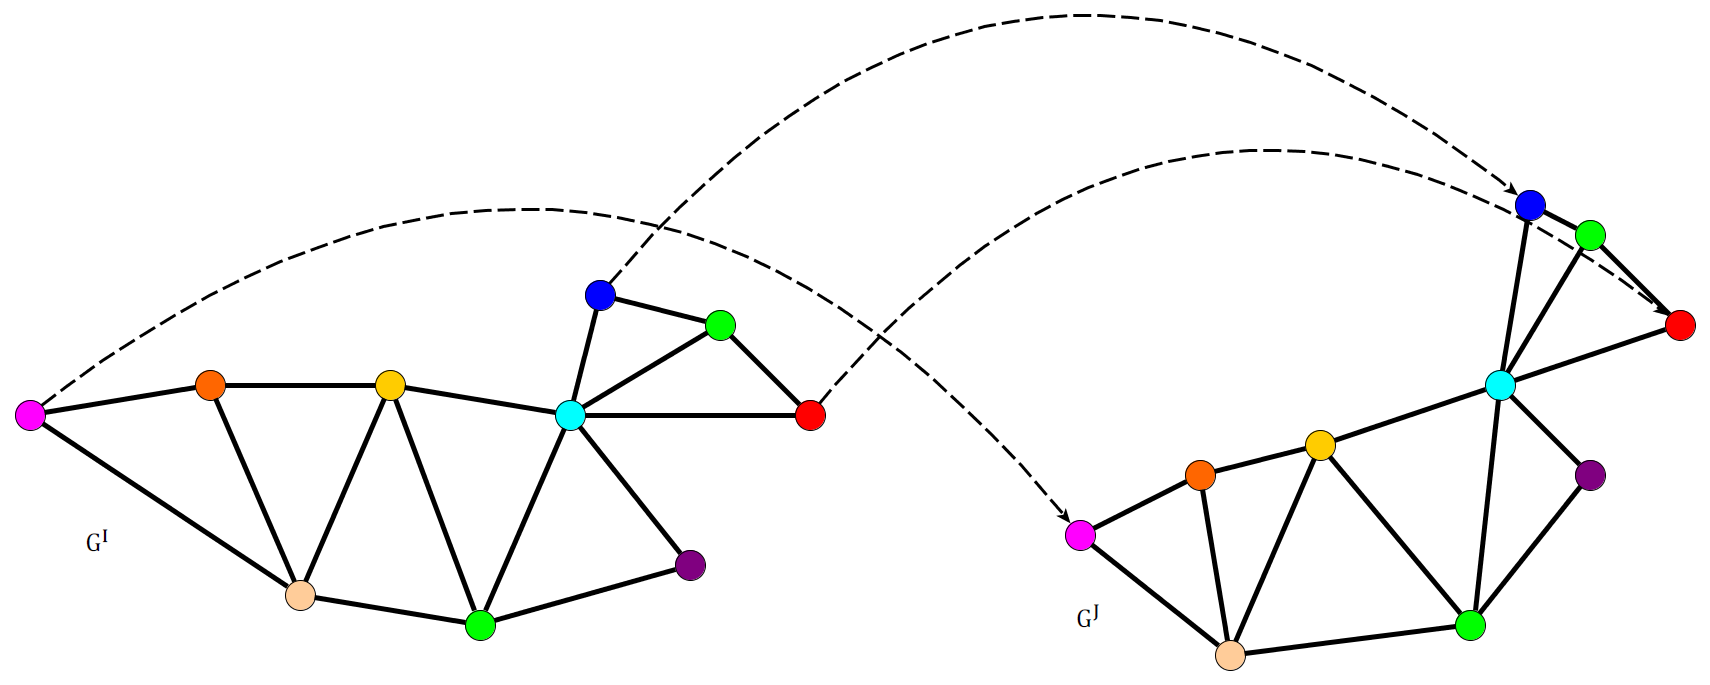
\includegraphics[width=10cm]{fig/duck1_duck2.png}
    \end{subfigure}
\end{figure}
\end{frame}

\begin{frame}
\frametitle{Goal}

\begin{figure}[h!]
    \centering
    \begin{subfigure}[b]{0.45\textwidth}
        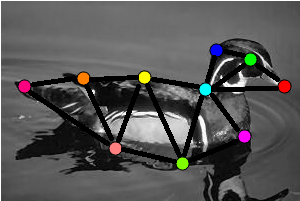
\includegraphics[width=\textwidth]{fig/duck1}
    \end{subfigure}
    \begin{subfigure}[b]{0.45\textwidth}
        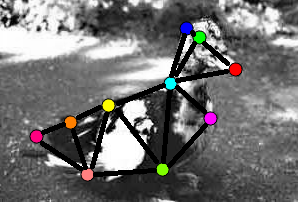
\includegraphics[width=\textwidth]{fig/duck2}
    \end{subfigure}
\end{figure}

\end{frame}
%--------------------------------------------------------------------------%
\begin{frame}
%\frametitle{Graph Matching}
Given two attributed graphs $\bar{G}^P=(\bar{V}^P, \bar{E}^P, \bar{A}^P)$ and $\bar{G}^Q=(\bar{V}^Q, \bar{E}^Q, \bar{A}^Q)$ with $n^P$ and $n^Q$ nodes respectively.

A result of graph matching is a subset of possible correspondences between those graphs, which can be represented in form of assignment matrix $X\in\{0,1\}^{n^P\times n^Q}$:
$$X_{ia} = \begin{cases} 1 & \mbox{node}\ v_i\in \bar{V}^P \mbox{matches}\ v_a \in \bar{V}^Q \\
						 0 & \mbox{otherwise} \\
			\end{cases}$$
General formulation:
$$x^* = \arg\max S(x)$$
$$ s.t. \begin{cases}
									x\in\{0,1\}^{n^Pn^Q} \\
								 \sum_{i=1}^{n^P}x_{ia}\le 1 \\
								 \sum_{a=1}^{n^Q}x_{ia}\le 1  \end{cases}$$
The objective function $S(x)$ measures the similarity between the graph attributes. 
\end{frame} 

%--------------------------------------------------------------------------%
%--------------------------------------------------------------------------%
\section{Solution techniques} 
\begin{frame}
\frametitle{Drei exemplarische Typen von Suchanfragen}
\begin{itemize}
\item spezielle: \hspace{50pt}
						\visible<2->{\textcolor{red}{Problem der Knappheit}} \\
	\glqq Does Netscape support the JDK 1.1 - code-signing API?\grqq
	\cite{Kleinberg}
	\begin{block}{}
	\item 
	breit angelegte: \hspace{30pt} 	
					\visible<3->{\textcolor{red}{Problem der Vielfältigkeit}} \\
	\glqq Find information about the Java programming language\grqq \cite{Kleinberg}
	\end{block}
	
	\item Suche nach ähnlichen Seiten\\
	\glqq Find pages similar to {\it java.sun.com}\grqq\cite{Kleinberg}
	
\end{itemize}
\end{frame}
%--------------------------------------------------------------------------%
\begin{frame}
\frametitle{Ranking}

\begin{itemize}
\item Man möchte die angesehensten Seiten (Authorities) aus der Menge aller zu der Anfrage relevanten Seiten finden
\item Mögliche Hindernisse:
	\begin{itemize}
	\item die höchst relevanten Seiten werden nicht unbedingt durch ein textbasiertes Ranking vorgezogen
	\item es kann sein,  dass die relevanten Seiten die Wörter aus der Suchanfrage gar nicht enthalten
	\end{itemize}
\end{itemize}
\end{frame}
%--------------------------------------------------------------------------%
\begin{frame}[allowframebreaks]

\begin{block}{Annahme}
Die Relevanz zwischen zwei Seiten wurde vom Ersteller des Links zwischen diesen Seiten geprüft
\end{block}

Stimmt im Allgemeinen nicht (z.B. Navigationslinks, Werbung)
\vspace{10pt}

Aber unter dieser Annahme reicht es, nur die Linkstruktur des WWW zu betrachten, um die Autorität einer Seite im Bezug auf eine andere zu bestimmen

\frametitle{Authorities und Hubs}

\framebreak

\begin{block}{Authorities (Autoritätsseiten)}
Relevante Seiten, auf die viele weitere relevante Seiten zeigen
\end{block}

%\vspace{5pt}
%\begin{minipage}[0.2\textheight]{\textwidth}
%	\begin{columns}[T]
%		\begin{column}{0.7\textwidth}
%			{\bf Problem}: populäre Seiten kommen immer als Authorities vor
%			
%			\vspace{10pt}
%			Es muss eine Überlappung in den Links, die auf Authorities zeigen, berücksichtigt werden
%		\end{column}
%		\begin{column}{0.2\textwidth}
%			\begin{figure}
%			\begin{tikzpicture}
%				\node[] (h) at ( 1.0, 1.3) {Hubs};
%				\node[] (v3) at ( 0.0, 0.0) {};\fill[red] (v3) circle (2pt);
%				\node[] (v4) at ( 1.0, 0.0) {};\fill[red] (v4) circle (2pt);
%				\node[] (v5) at ( 2.0, 0.0) {};\fill[red] (v5) circle (2pt);
%			
%				\node[] (v0) at ( 0.0, 1.0) {};\fill[blue] (v0) circle (2pt);
%				\node[] (v1) at ( 1.0, 1.0) {};\fill[blue] (v1) circle (2pt);
%				\node[] (v2) at ( 2.0, 1.0) {};\fill[blue] (v2) circle (2pt);
%				
%				\draw[->] (v2) to node[right] {} (v4);
%				
%				\draw[->] (v0) to node[right] {} (v3);
%				\draw[->] (v0) to node[right] {} (v5);
%				
%				\draw[->] (v1) to node[right] {} (v3);
%				\draw[->] (v1) to node[right] {} (v4);
%				
%				\node[] (a) at ( 1.0, -.2) {Authorities};
%			\end{tikzpicture}
%			\end{figure}
%		\end{column}
%	\end{columns}
%\end{minipage}

\begin{block}{Hubs}
Seiten, die auf viele Authorities zeigen
\end{block}

\end{frame}
%--------------------------------------------------------------------------%
%--------------------------------------------------------------------------%
\section{2LevelGM} 


%--------------------------------------------------------------------------%
%--------------------------------------------------------------------------%
\section{Evaluation} 

%--------------------------------------------------------------------------%
%--------------------------------------------------------------------------%
\section*{The End}
\begin{frame}{The end}
\centering
\LARGE
\color{red}
Thank you for your attention!
%\nocite{Kleinberg}
%\nocite{ZheZhao2}
%\nocite{CIS}
%\nocite{HITS_Lecture4_Cornell}
%\nocite{BeamerTheme} 
\nocite{Cho_LearningG}
\end{frame}
%--------------------------------------------------------------------------%
\begin{frame}
\centering
\begin{figure}
	
\includegraphics{who.png}
\end{figure}
\end{frame}
%--------------------------------------------------------------------------%
\begin{frame}[allowframebreaks]
	\frametitle{References}
	\bibliographystyle{plain}
	\bibliography{bibliographie}
\end{frame} 

\end{document}
%--------------------------------------------------------------------------%
%--------------------------------------------------------------------------%
%--------------------------------------------------------------------------%
